\documentclass[tikz,border=2pt]{standalone}
\usepackage{amsmath,amssymb}
\usepackage{pgfplots}
\pgfplotsset{compat=1.18}

\begin{document}
% A density is not a probability: probabilities are AREAS under it. The shaded region is
% P(a <= X <= b); the total area is 1 and the density itself may exceed 1.
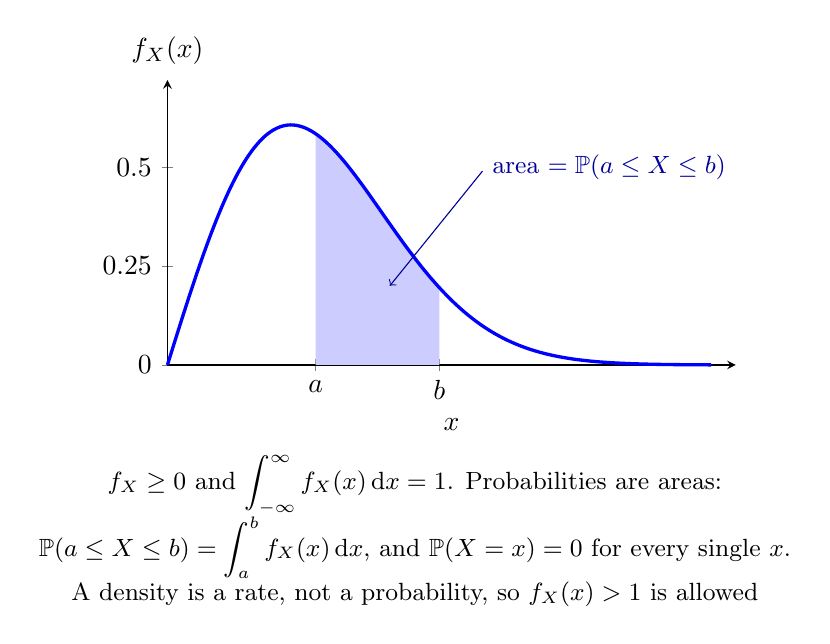
\begin{tikzpicture}
	\begin{axis}[
		axis lines=left, xmin=0, xmax=4.6, ymin=0, ymax=0.72,
		xtick={1.2,2.2}, xticklabels={$a$,$b$}, ytick={0,0.25,0.5},
		xlabel={$x$}, ylabel={$f_X(x)$}, ylabel style={rotate=-90, anchor=south, at={(axis description cs:0,1.02)}},
		samples=160, smooth, width=8.8cm, height=5.2cm, clip=false
		]
		\addplot[fill=blue!20, draw=none, domain=1.2:2.2] {x*exp(-x^2/2)} \closedcycle;
		\addplot[blue, very thick, domain=0:4.4] {x*exp(-x^2/2)};
		\node[blue!60!black, font=\small, anchor=west] at (axis cs:2.55,0.5) {area $=\mathbb{P}(a\le X\le b)$};
		\draw[blue!60!black, ->] (axis cs:2.55,0.49) -- (axis cs:1.8,0.2);
	\end{axis}
	\node[anchor=north, font=\small, align=flush center, text width=9.6cm] at ([yshift=-2pt]current axis.outer south) {$f_X\ge0$ and $\displaystyle\int_{-\infty}^{\infty}f_X(x)\,\mathrm{d}x=1$. Probabilities are areas: $\mathbb{P}(a\le X\le b)=\displaystyle\int_a^bf_X(x)\,\mathrm{d}x$, and $\mathbb{P}(X=x)=0$ for every single $x$. A density is a rate, not a probability, so $f_X(x)>1$ is allowed};
\end{tikzpicture}
\end{document}
